\chapter{Produto vetorial}

O produto vetorial de dois vetores $\vec{u}\times \vec{v}$ apresenta como resultado um vetor, ao contrário do que acontece com o produto escalar $\vec{u}\cdot \vec{v}$ que resulta em um escalar (número real).

\begin{df} Dados os vetores $\vec{u}=(x_1, y_1, z_1)$ e $\vec{v}=(x_2, y_2, z_2)$, chama-se produto vetorial de $\vec{u}$ por $\vec{v}$, nesta ordem, ao vetor representado por $\vec{u}\times \vec{v}$ e calculado por:$$\vec{u}\times \vec{v}= \left|
\begin{array}{ccc}
\vec i & \vec j & \vec k \\
x_1 & y_1 & z_1 \\
x_2 & y_2 & z_2 \\
\end{array}
\right|$$

O produto vetorial não está definido no $\mathbb{R}^2$.
\end{df} 

\section{Propriedades do produto vetorial}
\begin{enumerate}[(1)]
 \item $\vec{u}\times \vec{u}=0$
 \item $\vec{u}\times \vec{v}=-\vec{v}\times \vec{u}$
 \item $\vec{u}\times (\vec{v}+\vec{w})=\vec{u}\times \vec{v}+\vec{u}\times \vec{w}$
 \item $\alpha (\vec{u}\times \vec{v})=(\alpha \vec{u})\times \vec{v}=\vec{u} \times (\alpha \vec{v})$, com $\alpha \in \mathbb{R}$
 \item $\vec{u}\times \vec{v}=0$ se e somente se, um dos vetores é nulo ou os dois são colineares.
 \item \label{prop}$\vec{u}\times \vec{v}$ é simultaneamente ortogonal aos vetores $\vec{u}$ e $\vec{v}$ e o sentido de $\vec{u}\times \vec{v}$ é  dado  pela  \textit{regra da mão direita} ou pela \textit{regra do saca rolhas}.
 \begin{figure}[H]
 \centering
 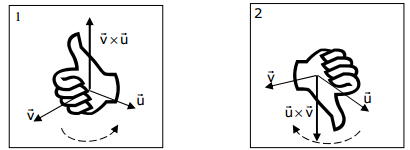
\includegraphics[width=0.4\linewidth]{analitica/imagens/rmd.png}
 \end{figure}
 
 \item $\vec{u} \times \vec{v} = \Vert \vec{u} \Vert \cdot \Vert \vec{v} \Vert \cdot \sin{\theta}$, onde $\theta$ é o ângulo entre os vetores $\vec{u}$ e $\vec{v}$.
\begin{figure}[H]
\centering
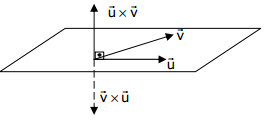
\includegraphics[width=0.4\linewidth]{analitica/imagens/prop.png}
\end{figure}
\end{enumerate}

\textbf{Importante:} Da propriedade (\ref{prop}), $\vec{u} // \vec{v} \quad \Leftrightarrow \quad \vec{u} \times \vec{v}=0$

\section{Interpretação geométrica do módulo do produto vetorial}

O módulo do produto vetorial de dois vetores $\vec u$ e $\vec v$ é igual a área do paralelogramo cujos lados são determinado pelos vetores $\vec u$ e $\vec v$.

\begin{figure}[H]
\centering
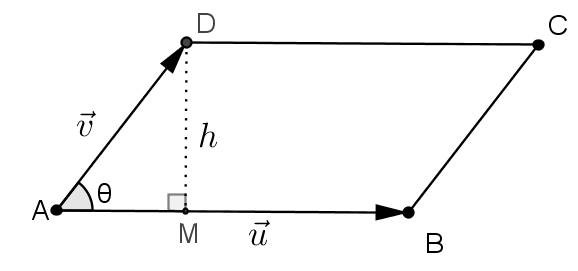
\includegraphics[width=0.4\linewidth]{analitica/imagens/prodvet.png}
\end{figure}

\textbf{Demonstração}: observe inicialmente que o paralelogramo $ABCD$ é determinado pelos vetores $\vec u=\overrightarrow{AB}$ e $\vec v=\overrightarrow{AD}$. Note que a altura do paralelogramo é dada por $h=\Vert v\Vert\cdot \sin{\theta}$

Em todo paralelogramo, a área é dada pela multiplicação da base pela altura, portanto:
\begin{eqnarray*}
A_{ABCD} & = & \Vert\vec u\Vert\cdot h \\
A_{ABCD} & = & \Vert\vec u\Vert\cdot \Vert v\Vert\cdot \sin{\theta} \\
A_{ABCD} & = & \Vert \vec u \times v \Vert
\end{eqnarray*}

Também é possível verificar que a área do triângulo $ABD$ é $$ A_{ABD}= \frac{\Vert\vec u \times v \Vert}{2}$$